\chapter{\difficult{Higher-dimensional Algebra}}\label{chapter:hda}

    The main reference for this chapter is the series of papers carrying the same name by \textit{Baez et al.} \cite{HDA5, HDA6}. References for the section on Berezin calculus are \cite{losev_berezin, AMP2}. For Kapranov-Voevodsky 2-vector spaces the reader is referred to the original paper \cite{kapranov_voevodsky}. The section about higher Lie theory is mainly based on \cite{bv_formalism}. For fusion and modular categories the main reference is \cite{etingof}.

\section{Graded vector spaces}\label{section:graded_spaces}

    \newdef{Graded vector space}{\index{degree!of vector}\index{graded!vector space}\label{hda:graded_vector_space}
        A vector space $V$ that can be decomposed as
        \begin{gather}
            V = \bigoplus_{i\in I}V_i
        \end{gather}
        for a collection of vector spaces $\{V_i\}_{i\in I}$, where $I$ can be both finite or countable. The index $i$ is often called the \textbf{degree} of the subspace $V_i$ in $V$. One writes $\deg(v)=i$ if $v\in V_i$.
    }
    \newdef{Finite type}{\index{finite!type}
        A graded vector space is said to be of finite type if it is finite-dimensional in each degree.
    }

    \begin{example}[Super vector space]\index{super-!vector space}\label{hda:superspace}
        A $\mathbb{Z}_2$-graded vector space.
    \end{example}

    \newdef{Graded algebra}{\index{graded!algebra}
        A $\mathbb{Z}$-graded vector space $V$ with the additional structure of an algebra $(V,\star)$ such that $V_k\star V_l\subseteq V_{k+l}$ for all $k,l\in\mathbb{Z}$.\footnote{The grading can be relaxed to any commutative monoid.}
    }
    \newdef{Graded-commutative algebra}{\index{graded!commutativity}\label{hda:graded_commutative}
        A graded algebra $(V,\star)$ such that
        \begin{gather}
            v\star w = (-1)^{\deg(v)\deg(w)}w\star v
        \end{gather}
        holds for all homogeneous elements $v,w\in V$.
    }

    \begin{example}[Superalgebra]\index{super-!algebra}\label{hda:superalgebra}
        A $\mathbb{Z}_2$-graded algebra
        \begin{gather}
            A = A_0\oplus A_1,
        \end{gather}
        such that for all $i,j$:
        \begin{gather}
            A_i\star A_j \subseteq A_{i+j\bmod2}.
        \end{gather}
    \end{example}

    \newdef{Parity and suspension}{\index{parity!functor}\index{suspension}
        Consider the category $\mathbf{sVect}$ of super vector spaces. One can define the \textbf{parity functor} $\func{\Pi}{sVect}{sVect}$ as the functor that interchanges even and odd subspaces:
        \begin{align}
            (\Pi V)_0 &:= V_1,\\
            (\Pi V)_1 &:= V_0.
        \end{align}
        A more general construction exists in $\mathbb{Z}$-$\mathbf{Vect}$. For every graded vector space $V$, the $k$-\textbf{shifted} vector space or $k$-\textbf{suspension} $V[k]$ is defined as follows (some authors use the opposite convention):
        \begin{gather}
            V[k]_i := V_{i-k}.
        \end{gather}
    }

    \begin{example}[Free GCA]\label{hda:symmetric_algebra}\index{word!length}
        Let $V$ be a graded vector space. The free GCA $\Sym^\bullet V$ on $V$ is defined as the quotient of the tensor algebra $T(V)$ by the relations
        \begin{gather}
            x\otimes y - (-1)^{\deg(x)\deg(y)}y\otimes x
        \end{gather}
        ranging over all homogeneous elements $x,y\in V$. (The notation stems from the fact that it is inherited from the symmetric monoidal structure on $\mathbf{Ch}_\bullet(\mathbf{Vect})$.) This algebra can equivalently be obtained as the tensor product
        \begin{gather}
            \Sym^\bullet V = \Sym(V_\mathrm{even})\otimes\Alt(V_\mathrm{odd}),
        \end{gather}
        where $\Sym$ and $\Lambda$ denote the symmetric and exterior algebras of ordinary vector spaces. It it not hard to see that this definition combines the definitions of $\Sym$ and $\Alt$ (for this reason it is sometimes also denoted by $\Sym^\bullet V$). A similar definition gives a graded alternating algebra:
        \begin{gather}
            \Alt^\bullet V = T(V)/(x\otimes y - (-1)^{\deg(x)\deg(y)}y\otimes x).
        \end{gather}
        Note that both of these algebras actually carry a bigrading, the total degree coming from $V$ and the \textbf{word length}:
        \begin{align}
            \deg(v_1\cdots v_n) &:= \deg(v_1)+\cdots+\deg(v_n)\\
            \mathrm{wl}(v_1\cdots v_n) &:= n.
        \end{align}
        In general, only the word length is made explicit when writing down the space, i.e. $v\in\Alt^{\mathrm{wl}(v)}V$.
    \end{example}
    \begin{remark}[Different conventions and d\'ecalage]\index{d\'calage}\index{Koszul!sign}\label{hda:decalage}
        Some authors use the notation $\Lambda^\bullet V$ for the free graded-commutative algebra on $V$. However, this might be confused with the notation for the Grassmann (exterior) algebra of an ordinary vector space.\footnote{This inconvenient change of conventions can be found everywhere in the literature, so one should pay close attention to the conventions that are used.} In fact, there is a good reason why these notations are used in a seemingly interchangeable way for graded vector spaces. The suspension functor $V\rightarrow V[1]$ gives a way to relate the Grassmann algebra over an ordinary vector space $V$ to the free GCA on the shifted space $V[1]$, i.e. $\Alt^\bullet V\cong\Sym^\bullet V[1]$. However, at this point, the \textbf{d\'ecalage isomorphism}
        \begin{gather}
            \mathrm{dec}_k:\Lambda^kV[k]\cong\Sym^kV[1]
        \end{gather}
        is only a linear isomorphism. There are two ways to see that it can be extended to an algebra isomorphism.

        The first one defines the suspension functor as an intertwiner between the symmetrization and antisymmetrization operations to define $\Sym$ and $\Alt$. Define the symmetric and antisymmetric Koszul signs of a permutation $\sigma\in S_n$ as follows:
        \begin{align}
            \varepsilon(\sigma;v_1,\ldots,v_n) &:= (-1)^{\#\text{ odd-odd neighbour transpositions in }\sigma}\\
            \chi(\sigma;v_1,\ldots,v_n) &:= \sgn(\sigma)\varepsilon(\sigma;v_1,\ldots,v_n).
        \end{align}
        D\'ecalage then says that the suspension functor should satisfy
        \begin{gather}
            \varepsilon(\sigma;v_1,\ldots,v_n)\sigma\circ[1]^{\otimes n} = [1]^{\otimes n}\circ\chi(\sigma;v_1,\ldots,v_n)\sigma.
        \end{gather}
        Since both $\Sym$ and $\Alt$ can be defined in terms of the projectors
        \begin{gather}
            p_{\Sym}:=\sum_{\sigma\in S_n}\varepsilon(\sigma)\sigma\qquad\text{and}\qquad p_{\Alt}:=\sum_{\sigma\in S_n}\chi(\sigma)\sigma,
        \end{gather}
        d\'ecalage interchanges symmetric and antisymmetric tensors. The most common choice is the following one:
        \begin{gather}
            [1]:V^{\otimes n}\rightarrow V[1]^{\otimes n}:v_1\otimes\cdot\otimes v_n\mapsto(-1)^{\sum_{i=1}^n(n-i)\deg(v_i)}v_1[1]\otimes\cdots\otimes v_n[1].
        \end{gather}
        This choice is induced by the following definition of the suspension functor (one could also choose the convention where $V$ is tensored on the right):
        \begin{gather}
            [1]:\mathbb{Z}\text{-}\mathbf{Vect}_k\rightarrow\mathbb{Z}\text{-}\mathbf{Vect}_k:V\mapsto k[1]\otimes V.
        \end{gather}
        This definition also directly induces an algebra isomorphism in the following way. Consider two homogeneous elements $v,w\in V$. In $\Sym^2V$ their product satisfies \[vw = (-1)^{\deg(v)\deg(w)}wv.\] After applying the suspension functor, the product on the left-hand side becomes: \[v[1]w[1]\equiv(\underline{1}\otimes v)(\underline{1}\otimes w) \cong (-1)^{\deg(w)}\underline{\underline{1}}\otimes(vw)\equiv(-1)^{\deg(w)}vw[2].\] To calculate the suspension of the right-hand side, the braiding in $\mathbb{Z}\text{-}\mathbf{Vect}_k$ is used:
        \begin{align*}
            v[1]w[1]\equiv(v\otimes\underline{1})(w\otimes\underline{1})\mapsto&(-1)^{\deg(v)+\deg(w)+\deg(v)\deg(w)+1}(w\otimes\underline{1})(v\otimes\underline{1})\\
            =&(-1)^{\deg(w)+\deg(v)\deg(w)+1}(wv)\otimes\underline{\underline{1}}\\
            \equiv&(-1)^{\deg(w)+\deg(v)\deg(w)+1}wv[2].
        \end{align*}
        The difference in signs is $(-1)^{\deg(v)\deg(w)+1}$. If either $v$ or $w$ is even, this final sign is $-1$ or equivalently, the product is antisymmetric, while if both $v$ and $w$ are odd, the product is symmetric. This is exactly the opposite situation of that in $\Sym^2V$. The most thorough review of these issues was found in \cite{MitiAntonioMichele2021Hcmi}.
    \end{remark}

\subsection{Supermatrices}

    For this section the requirement that all algebraic structures are defined over a field $K$ is relaxed to working over a supercommutative ring. This means that the objects will be (graded) modules instead of proper vector spaces.

    \newdef{Supermatrix}{\index{parity!of matrix}
        Every linear transformation between super vector spaces $(V_0,V_1)$ and $(W_0,W_1)$ can be decomposed as the sum of 4 linear transformations between the even/odd subspaces:
        \begin{itemize}
            \item $A:V_0\rightarrow W_0$,
            \item $B:V_1\rightarrow W_0$,
            \item $C:V_0\rightarrow W_1$, and
            \item $D:V_1\rightarrow W_1$.
        \end{itemize}
        If these components are represented as matrices, the full transformation can be represented as a block matrix \[X=\begin{pmatrix}A&B\\C&D\end{pmatrix}.\]

        These matrices can be classified according to their \textbf{parity}. Not all supermatrices preserve the grading or, equivalently, not all linear transformations of super vector spaces are morphisms of super vector spaces. The ones that are, are said to have even parity and they are of the form \[X=\begin{pmatrix}\mathrm{even}&\mathrm{odd}\\\mathrm{odd}&\mathrm{even}\end{pmatrix},\] where even/odd means that the entries in these blocks have even/odd parity as elements of the underlying (graded) ring. It should be clear that these matrices indeed preserve the grading, since acting with an odd scalar on an odd vector gives an even vector (and similarly for the other combinations). The matrices that do not preserve the grading are said to have odd parity and are of the form \[X=\begin{pmatrix}\mathrm{odd}&\mathrm{even}\\\mathrm{even}&\mathrm{odd}\end{pmatrix}.\]
    }

    \newdef{Supertrace}{\index{super-!trace}
        The supertrace of a supermatrix generalizes the trace of an ordinary matrix. Given the block matrix form from the previous definition, the supertrace is defined as follows:
        \begin{gather}
            \mathrm{str}(X) := \tr(A)-\tr(D).
        \end{gather}
    }
    \begin{property}
        As was the case for the ordinary trace, the supertrace is invariant under basis transformations. Furthermore, the cyclicity property also still holds after a slight modification to make it compatible with the grading:
        \begin{gather}
            \mathrm{str}(XY) = (-1)^{\deg(X)\deg(Y)}\mathrm{str}(YX).
        \end{gather}
    \end{property}

    \newdef{Berezinian}{\label{hda:berezinian}
        The Berezinian or \textbf{superdeterminant} generalizes the determinant of an ordinary matrix. It is (uniquely) defined through the following two conditions:
        \begin{enumerate}
            \item $\mathrm{Ber}(XY) = \mathrm{Ber}(X)\mathrm{Ber}(Y)$, and
            \item $\mathrm{Ber}(e^X) = e^{\mathrm{str}(X)}$.
        \end{enumerate}
        An explicit formula is given by
        \begin{gather}
            \mathrm{Ber}(X) = \det(A - BD^{-1}C)\det(D)^{-1} = \det(A)\det(D-CA^{-1}B)^{-1},
        \end{gather}
        where the last expression involves the \textit{Schur complement} of $A$ relative to $X$. It should be noted that the Berezinian is only well-defined for invertible even matrices.
    }

\subsection{Berezin calculus}\label{section:berezin}

    This section is an application of the concept of exterior algebras \ref{vector:exterior_algebra}. Grassmann numbers/variables are used in quantum field theory when performing calculations in e.g. the fermionic sector or \textit{Faddeev-Popov quantization}.

    \newdef{Grassmann numbers}{\index{Grassmann!number}\label{hda:grassmann_number}
        Let $V$ be a vector space spanned by a set of elements $\theta_i$. The Grassmann algebra with Grassmann variables $\theta_i$ is the exterior algebra over $V$. In this setting the wedge symbol of Grassmann variables is often ommitted when writing the product: \[\theta_i\wedge\theta_j \equiv \theta_i\theta_j.\]
    }
    \begin{remark}
        From the (anti)commutativity it follows that one can regard the Grassmann variables as being nonzero square roots of zero.
    \end{remark}

    \begin{notation}[Parity]\index{parity}
        In the case of superalgebras and, in particular, that of Grassmann numbers, the degree of an element is often called the (Grassmann) parity of the element. It is also often denoted by $\varepsilon(x)$ or $\varepsilon_x$ instead of $\deg(x)$. In this text this convention is only adopted for graded algebras where there is both a supergrading and a (co)homological $\mathbb{Z}$-grading.
    \end{notation}

    \begin{property}[Polynomials]
        Consider a one-dimensional Grassmann algebra (with generator $\theta$). When constructing the polynomial ring $\mathbb{C}[\theta]$ generated by $\theta$, it can be seen that, due to the anticommutativity, $\mathbb{C}[\theta]$ is spanned only by $1$ and $\theta$. All higher-degree terms vanish because $\theta^2 = 0$. This implies that the most general polynomial over a one-dimensional Grassmann algebra is of the form
        \begin{gather}
            p(\theta) = a + b\theta.
        \end{gather}
    \end{property}

    \begin{definition}\index{DeWitt!convention}
        One can equip the exterior algebra $\Lambda$ with Grassmann variables $\theta_i$ with an involution:
        \begin{gather}
            (\theta_i\theta_j\ldots\theta_k)^* := \theta_k\ldots\theta_j\theta_i.
        \end{gather}
        Elements $z\in\Lambda$ that satisfy $z^*=z$ are said to be \textbf{(super)real} and elements thar satisfy $z^*=-z$ are said to be \textbf{(super)imaginary}. This convention is called the \textbf{DeWitt convention}.
    \end{definition}

    To keep the discussion about Grassmann variables self-contained, the calculus of Grassmann variables is introduced here:
    \newdef{Derivative of Grassmann variables}{
        Consider the polynomial algebra $\mathbb{C}[\theta_1,\ldots,\theta_n]$ on $n$ Grassmann variables (more general functions would be defined through a series expansion, but given that $\theta^2=0$, these always reduce to a simple polynomial). Differentiation on this ring is defined through the following relations:
        \begin{gather}
            \pderiv{}{\theta_j}\theta_i = \delta_i^j\qquad\qquad\qquad\theta_i\pderiv{}{\theta_j}+\pderiv{}{\theta_j}\theta_i = 0
        \end{gather}
        The second relation implies that the partial derivatives are also Grassmann-odd. The odd parity in fact allows to introduce two distinct differentiation operations. One is the left derivative, this is the one that was just introduced. The other is the right derivative that acts as
        \begin{gather}
            \theta_i\pderiv{^R}{\theta^j} = \delta_i^j.
        \end{gather}
        The left and right derivatives are also sometimes denoted by \[\overset{\rightarrow}{\pderiv{}{\theta^i}} \qquad\qquad\text{and}\qquad\qquad \overset{\leftarrow}{\pderiv{}{\theta^i}},\] respectively.
    }

    Next, one also needs some kind of integration theory. Instead of working with a definition \`a la Riemann, the integral will be defined purely axiomatically:
    \newdef{Berezin integral: axiomatic}{\index{Berezin!integral}
        Consider a function $f$ of $n$ Grassmann variables $\{\theta_i\}_{i\leq n}$. The Berezin integral $\int_B$ is defined by the following conditions:
        \begin{enumerate}
            \item The map $f\mapsto\int_Bf(\theta)d\theta$ is linear.
            \item The result $\int_Bf(\theta)d\theta$ is independent of the variable(s) $\theta$, i.e. it is a number.
            \item The result is invariant under a translation of the integration variable.
        \end{enumerate}
    }
    \begin{remark}
        Multiple integrals can be defined by adding the Fubini theorem as an additional axiom.
    \end{remark}

    It can be shown that this definition is equivalent to the following one:
    \newadef{Berezin integral: analytic}{
        First consider functions in one Grassmann variable, i.e. $f(\theta) = a+b\theta$. The Berezin integral is then defined as follows:\footnote{Technically the axioms only imply this formula up to some multiplicative constant. The original convention by \textit{Berezin} will be adopted, i.e. this constant is chosen to be $1$.}
        \begin{gather}
            \int_B(a+b\theta)d\theta := b.
        \end{gather}
        This means that the integral is equal to the coefficient of the highest-degree term. As a simple generalization, define
        \begin{gather}
            \int_Bf(\theta_1,\ldots,\theta_n)d\theta := \text{coefficient of }\theta_1\cdots\theta_n.
        \end{gather}
        Some authors reverse the order of the variables in the above definition. Depending on the number of variables, this might introduce an additional minus sign.
    }
    \begin{remark}
        It is interesting to see that the (one-dimensional) Berezin integral is equal to the (Grassmann) derivative. This is completely different from the usual integral in calculus. It also gives some intuition for the distinct transformation behaviour of the Berezin integral as explained in the following property.
    \end{remark}

    \begin{formula}[Change of variables]
        Consider a general Berezin integral $\int_Bf(\theta)d\theta$. Now, suppose that a transformation $\theta\rightarrow\xi(\theta)$ is applied to the Grassmann variables. If $J$ is the Jacobian matrix associated to this transformation, the integral transforms according to the following formula:
        \begin{gather}
            \int_Bf(\xi)d\xi = \int_Bf(\theta)(\det J)^{-1}d\theta.
        \end{gather}
    \end{formula}

    Berezin calculus can easily be unified with ordinary calculus by using the fact that ordinary coordinates (even parity) commute with Grassmann numbers (odd parity). A mixed derivative (resp. integral) can always be factorized as the composition of a Berezin derivative (resp. integral) and an ordinary one. The transformation behaviour is then generalized to this case by using the Berezinian \ref{hda:berezinian}.

\section{Monoidal categories II: Duality}\label{section:duality}

    The general theory of monoidal categories was introduced in Section \ref{section:monoidal_categories}.

    \newdef{Dual object}{\index{dual!object}\label{hda:dual}
        Let $(\mathbf{C},\otimes,\mathbf{1})$ be a monoidal category and consider an object $x\in\ob{C}$. A left dual\footnote{$x$ is called the \textbf{right dual} of $x^*$. The right dual of $y$ is often denoted by ${}^*y$.} of $x$ is an object in $x^*\in\ob{C}$ together with two morphisms $\eta:\mathbf{1}\rightarrow x\otimes x^*$ and $\varepsilon:x^*\otimes x\rightarrow\mathbf{1}$, called the \textbf{unit} and \textbf{counit} morphisms\footnote{Also called the \textbf{coevaluation} and \textbf{evaluation} morphisms.}, such that the diagrams in Figure \ref{fig:dual_objects} commute. $x$ is said to be \textbf{dualizable} if the object $x^*$ and the morphisms $\eta,\varepsilon$ exist.

        \begin{figure}[ht!]
            \centering
            \begin{subfigure}[b]{0.49\textwidth}
                \centering
                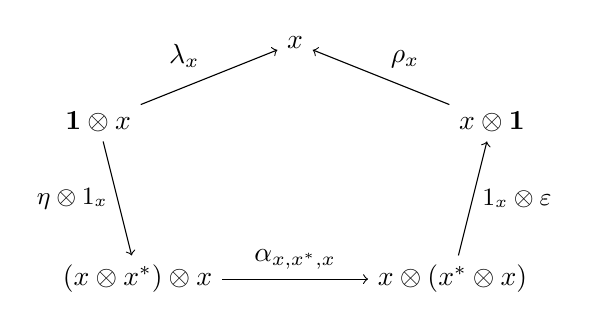
\begin{tikzpicture}
                    \node (X) at (0, 0) {$x$};
                    \node (1X) at (-2.5, -1) {$\mathbf{1}\otimes x$};
                    \node (X1) at (2.5, -1) {$x\otimes\mathbf{1}$};
                    \node (1XXX) at (-2, -3) {$(x\otimes x^*)\otimes x$};
                    \node (XXX1) at (2, -3) {$x\otimes(x^*\otimes x)$};
                    \draw[->] (1X) -- node[above left]{$\lambda_x$} (X);
                    \draw[->] (X1) -- node[above right]{$\rho_x$} (X);
                    \draw[->] (1X) -- node[left]{\small $\eta\otimes\mathbbm{1}_x$} (1XXX);
                    \draw[->] (XXX1) -- node[right]{\small $\mathbbm{1}_x\otimes\varepsilon$} (X1);
                    \draw[->] (1XXX) -- node[above]{$\alpha_{x,x^*,x}$} (XXX1);
                \end{tikzpicture}
                \caption{Dual object I.}
                \label{fig:dual_object1}
            \end{subfigure}
            \begin{subfigure}[b]{0.49\textwidth}
                \centering
                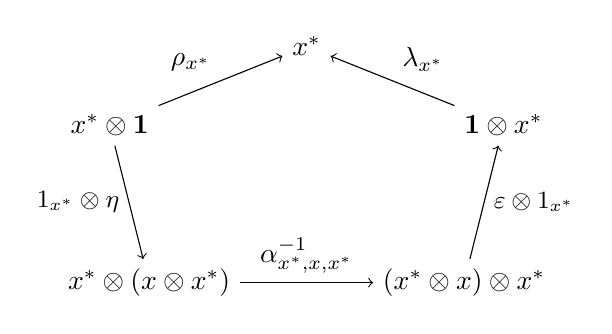
\begin{tikzpicture}
                    \node (X) at (0, 0) {$x^*$};
                    \node (X1) at (-2.5, -1) {$x^*\otimes\mathbf{1}$};
                    \node (1X) at (2.5, -1) {$\mathbf{1}\otimes x^*$};
                    \node (XXX1) at (-2, -3) {$x^*\otimes(x\otimes x^*)$};
                    \node (1XXX) at (2, -3) {$(x^*\otimes x)\otimes x^*$};
                    \draw[->] (X1) -- node[above left]{$\rho_{x^*}$} (X);
                    \draw[->] (1X) -- node[above right]{$\lambda_{x^*}$} (X);
                    \draw[->] (X1) -- node[left]{\small $\mathbbm{1}_{x^*}\otimes\eta$} (XXX1);
                    \draw[->] (1XXX) -- node[right]{\small $\varepsilon\otimes\mathbbm{1}_{x^*}$} (1X);
                    \draw[->] (XXX1) -- node[above]{$\alpha^{-1}_{x^*,x,x^*}$} (1XXX);
                \end{tikzpicture}
                \caption{Dual object II.}
                \label{fig:dual_object2}
            \end{subfigure}
            \caption{Dualizable objects.}
            \label{fig:dual_objects}
        \end{figure}
    }

    \newdef{Rigid category}{\index{category!rigid}\index{category!autonomous}
        A monoidal category that admits all duals. These categories are also said to be \textbf{autonomous}. If only left (resp. right) duals exist, the category is said to be left (resp. right) rigid.
    }

    \begin{property}[Braided categories]\label{hda:braided_rigid}
        In general it is not true that left and right duals coincide. However, in a braided monoidal category this is the case.
    \end{property}
    \newdef{Compact closed category}{\index{category!compact closed}
        A symmetric rigid category.
    }

    \begin{example}[FinVect]\index{dual!space}\index{resolution!of the identity}
        Consider the category $\mathbf{FinVect}$ of finite-dimensional vector spaces (the ground field is assumed to be $\mathbb{R}$). The categorical dual of a vector space $V$ is the algebraic dual $V^*$. The unit morphism is given by the ``resolution of the identity'':
        \begin{gather}
            \eta:\mathbf{1}\rightarrow V\otimes V^*:1\mapsto\sum_{i=1}^{\dim(V)}e_i\otimes\phi^i,
        \end{gather}
        where $\{e_i\}$ and $\{\phi^i\}$ are bases of $V$ and $V^*$, respectively.

        It should be noted that the category $\mathbf{Vect}$ of all vector spaces is not rigid. By Property \ref{hda:braided_rigid} above, left and right duals coincide in any braided monoidal category (such as $\mathbf{Vect}$). However for infinite-dimensional vector spaces it is known that $A\cong(A^*)^*$ never holds and as such rigidity cannot be extended to $\mathbf{Vect}$.
    \end{example}
    \begin{property}[Tannaka duality]\index{Tannaka duality}
        Consider the category $\mathcal{V}=\mathbf{FinVect}_K$. Using coends one can reconstruct the base field from its modules, i.e. the objects in $\mathcal{V}$:\footnote{This result can be shown to hold for all compact closed categories $\mathcal{V}$. In this context it is known as \textbf{Tannaka reconstruction}.}
        \begin{gather}
            \int^{V\in\mathcal{V}}V^*\otimes V\cong K.
        \end{gather}
        A more general statement goes as follows:
        \begin{gather}
            \int^{V\in\mathcal{V}}\mathcal{V}(V, -)\otimes\mathrm{id}_{\mathcal{V}}V\cong\mathrm{id}_{\mathcal{V}}.
        \end{gather}
        The components $\eta_V:\mathcal{V}(V,V)\rightarrow K$ of the coend can be shown to coincide with the trace and as such the trace obtains a universal property.
    \end{property}
    \remark{This property can also be generalized by replacing $\mathcal{V}$ by a category of modules $A\mathbf{Mod}$ for some finite-dimensional algebra $A$. The end and coend give respectively the algebra $A$ and its dual $A^*$.}

    The trace on $\mathbf{FinVect}$ can be generalized as follows:
    \newdef{Trace}{\index{trace!categorical}
        Let $(\mathbf{C},\otimes,\mathbf{1})$ be a rigid category and let $f\in\mathbf{C}(x,x^{**})$. The left (\textbf{categorical} or \textbf{quantum}) trace of $f$ is defined as the following morphism in $\End_{\mathbf{C}}(\mathbf{1})$:
        \begin{gather}
            \tr^L(f):=\varepsilon_{x^*}\circ(f\otimes\mathbbm{1}_{x^*})\circ\eta_x.
        \end{gather}
        For $f\in\mathbf{C}(x,{}^{**}x)$, the right trace is defined similarly:
        \begin{gather}
            \tr^R(f):=\varepsilon_{{}^{**}x}\circ(\mathbbm{1}_x\otimes f)\circ\eta_{{}^*x}.
        \end{gather}
    }
    \begin{property}
        The following linear algebra-like properties hold for the categorical trace:
        \begin{itemize}
            \item $\tr^L(f) = \tr^R(f^*)$,
            \item $\tr^L(f\otimes g) = \tr^L(f)\tr^L(g)$, and
            \item for additive categories: $\tr^L(f\oplus g) = \tr^L(f) + \tr^L(g)$.
        \end{itemize}
        The second and third property can be stated analogously for the right trace.
    \end{property}

    \newdef{Pivotal category}{\index{pivotal structure}
        Let $\mathbf{C}$ be a rigid monoidal category. A pivotal structure on $\mathbf{C}$ is a monoidal natural isomorphism $a_x:x\cong x^{**}$.
    }

    \newdef{Dimension}{\index{dimension!pivotal}
        Let $(\mathbf{C},a)$ be a pivotal category and consider an object $x\in\ob{C}$. The dimension of $x$ is defined as follows:
        \begin{gather}
            \label{hda:pivotal_dimension}
            \dim_a(x) := \tr^L(a_x).
        \end{gather}
    }

    \newdef{Spherical category}{\index{spherical structure}
        Let $(\mathbf{C},a)$ be a pivotal category. If the left and right traces with respect to $a$ coincide in $\mathbf{C}$, i.e. $\dim_a(x) = \dim_a(x^*)$, the pivotal structure is said to be spherical.
    }

    \newdef{Symmetric monoidal dagger category}{\index{category!dagger}
        A symmetric monoidal category $(\mathbf{C},\otimes,\mathbf{1})$ that also carries the structure of a dagger category \ref{cat:dagger_category} such that
        \begin{gather}
            (f\otimes g)^\dag = f^\dag\otimes g^\dag
        \end{gather}
        and such that the coherence and braiding morphisms are unitary.
    }
    \newdef{Dagger-compact category}{
        A symmetric monoidal dagger category that is also a compact closed category such that the following diagram commutes for all objects:
        \begin{gather*}
            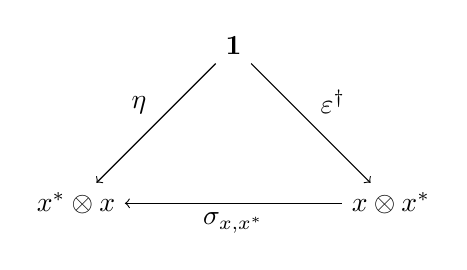
\begin{tikzpicture}
                \node (1) at (0, 0) {$\mathbf{1}$};
                \node (X*X) at (-2, -2) {$x^*\otimes x$};
                \node (XX*) at (2, -2) {$x\otimes x^*$};
                \draw[->] (1) -- node[above left]{$\eta$} (X*X);
                \draw[->] (1) -- node[above right]{$\varepsilon^\dagger$} (XX*);
                \draw[<-] (X*X) -- node[below]{$\sigma_{x,x^*}$} (XX*);
            \end{tikzpicture}
        \end{gather*}
    }

\section{Tensor and fusion categories}

    Some definitions might slightly differ from the ones in the main references and some properties might be stated less generally. $K$ denotes an algebraically closed field (often this will be $\mathbb{C}$).

    \newdef{Tensor category}{\index{tensor!category}
        A monoidal category with the following properties:
        \begin{enumerate}
            \item it is rigid,
            \item it is Abelian,
            \item it is $K$-linear (and it is so in a way compatible with the Abelian structure),
            \item $\End(\mathbf{1})\cong K$, and
            \item $-\otimes-$ is bilinear on morphisms.
        \end{enumerate}
        Some authors (such as \cite{etingof}) also add ``locally finite'' as a condition (Definition \ref{cat:locally_finite}).
    }
    \remark{If $K$ is not algebraically closed, one should exchange the last condition by the condition that $\mathbf{1}$ is a simple object. However, if $K$ is algebraically closed, these statements are equivalent.}

    \newdef{Pointed tensor category}{\index{pointed!tensor category}
        A tensor category where all of the simple objects are (weakly) invertible.
    }

    \newdef{Fusion category}{\index{fusion!category}
        A semisimple finite tensor category.
    }

    \begin{property}
        Let $\mathbf{C}$ be a fusion category. There exists a natural isomorphism $\mathbbm{1}_\mathbf{C}\cong\ast\ast$.
    \end{property}
    \begin{remark}
        Although any fusion category admits a natural isomorphism between an object and its double dual, this morphism does not need to be monoidal. The fact that all fusion categories are pivotal was conjectured by \textit{Etingof, Ostrik} and \textit{Nikshych}. Currently the best one can do for a general fusion category is a monoidal natural transformation between the identity functor and the fourth dualization functor $\mathbbm{1}_\mathbf{C}\cong\ast\ast\ast\ast$.
    \end{remark}

    \newdef{Categorical dimension}{\index{dimension!categorical}
        Consider a fusion category $\mathbf{C}$ and choose a natural isomorphism $a:\mathbbm{1}_\mathbf{C}\cong\ast\ast$. For every simple object $x$ one can define a dimension function, sometimes called the \textbf{norm squared}, in the following way:
        \begin{gather}
            |x|^2 := \tr(a_x)\tr((a_x^{-1})^*).
        \end{gather}
        If $\mathbf{C}$ is pivotal, this becomes $|x|^2 = \dim_a(x)\dim_a(x^*)$. In particular, when $\mathbf{C}$ is spherical, this becomes $|x|^2 = \dim_a(x)^2$.

        The categorical dimension, sometimes called the \textbf{M\"uger dimension}, is then defined as follows:
        \begin{gather}
            \dim(\mathbf{C}) := \sum_{x\in\mathcal{O}(\mathbf{C})}|x|^2,
        \end{gather}
        where $\mathcal{O}(\mathbf{C})$ denotes the set of isomorphism classes of simple objects.
    }
    \remark{It should be noted that the above quantities do not depend on the choice of isomorphism $a_x:x\cong x^{**}$ since all of them only differ by a scale factor.}
    \begin{property}[Nonzero dimension]
        For any fusion category $\mathbf{C}$ one has that $\dim(\mathbf{C})\neq 0$. In particular, if $K=\mathbb{C}$, then $\dim(\mathbf{C})\geq1$ (since the norm squared of any simple object is then also positive).
    \end{property}

    \newdef{$G$-graded fusion category}{\index{G-!grading}
        A semisimple linear category $\mathbf{C}$ is said to have a \textbf{$G$-grading}, where $G$ is a finite group, if it can be decomposed as follows:
        \begin{gather}
            \mathbf{C}\cong\bigoplus_{g\in G}\mathbf{C}_g,
        \end{gather}
        where every $\mathbf{C}_g$ is linear and semisimple. A fusion category $\mathbf{C}$ is said to be a ($G$-)graded fusion category if it admits a $G$-grading such that $\mathbf{C}_g\otimes\mathbf{C}_h\subset\mathbf{C}_{gh}$ for all $g,h\in G$.
    }

    \begin{example}[$G$-graded vector spaces]\label{hda:g_graded}
        Define the category $\mathbf{Vect}_G^\omega$ as having the same objects and morphisms as $\mathbf{Vect}_G$, the category of $G$-graded vector spaces, but with the associator given by the the 3-cocycle $\omega\in H^3(G;K^\times)$.
    \end{example}
    \begin{property}
        Any pointed fusion category is equivalent to a category of the form $\mathbf{Vect}_G^\omega$ for some $G$ and $\omega\in H^3(G;K^\times)$.
    \end{property}

    \begin{theorem}[Tannaka duality]\index{Tannaka duality}
        The category of modules of a weak Hopf algebra has the structure of a fusion category. Conversely, any fusion category can be obtained as the category modules of a weak Hopf algebra.
    \end{theorem}

\section{Ribbon and modular categories}

    \newdef{Ribbon structure}{
        Consider a braided monoidal category $(\mathbf{C},\otimes,\mathbf{1})$ with braiding $\sigma$. A \textbf{twist} or \textbf{balancing} is a natural transformation $\theta$ such that the following equation is satisfied for all $x,y\in\ob{C}$:
        \begin{gather}
            \theta_{x\otimes y} = (\theta_x\otimes\theta_y)\circ\sigma_{y,x}\circ\sigma_{x,y}.
        \end{gather}
        If in addition $\mathbf{C}$ is rigid and the twist satisfies $\theta_{x^*} = (\theta_x)^*$ for all $x\in\ob{C}$, one speaks of a ribbon category.
    }

    \newdef{Drinfel'd morphism}{\index{Drinfel'd!morphism}
        Let $(\mathbf{C},\otimes,\mathbf{1})$ be a rigid braided monoidal category with braiding $\sigma$. This structure admits a canonical natural isomorphism $x\cong x^{**}$ defined as follows:
        \begin{gather}
            x\xrightarrow{\mathbbm{1}_x\otimes\eta_{x^*}}x\otimes x^*\otimes x^{**}\xrightarrow{\sigma_{x,x^*}\otimes\mathbbm{1}_{x^{**}}}x^*\otimes x\otimes x^{**}\xrightarrow{\varepsilon_x\otimes\mathbbm{1}_{x^{**}}}x^{**}.
        \end{gather}
    }
    \begin{property}
        Let $\mathbf{C}$ be a braided monoidal category. Consider the canonical natural isomorphism $u_x:x\cong x^{**}$ defined above. Any natural isomorphism $\psi_x:x\cong x^{**}$ can be written as $u_x\theta_x$ where $\theta\in\Aut(\mathbbm{1}_\mathbf{C})$. It is not hard to see that this natural isomorphism is monoidal (hence pivotal) exactly when $\theta$ is a twist. If $\mathbf{C}$ is a fusion category then the pivotal structure is spherical if and only if $\theta$ gives a ribbon structure.
    \end{property}

    \newdef{Premodular category}{
        A ribbon fusion category. Equivalently, a spherical braided fusion category.
    }
    \newdef{$S$-matrix}{\index{S-matrix}
        Given a premodular category $\mathbf{M}$ (with braiding $\sigma$) one defines the $S$-matrix as follows:
        \begin{gather}
            S_{x,y} := \tr(\sigma_{y,x}\circ\sigma_{x,y}),
        \end{gather}
        where $x,y\in\mathcal{O}(\mathbf{M})$ are (isomorphism classes of) simple objects.

        Since in a premodular category there are only finitely many isomorphism classes of simple objects (denote this number by $\mathcal{I}$), one can see that $S$ is a $\mathcal{I}\times\mathcal{I}$-matrix.
    }

    \newdef{Modular category\footnotemark}{\index{modular!category}
        \footnotetext{``Modular tensor category'' is often abbreviated as \textbf{MTC}.}
        \nomenclature[A_MTC]{MTC}{modular tensor category}
        A premodular category for which the $S$-matrix is invertible.
    }

    \begin{property}
        Let $\mathbf{M}$ be a modular category with $S$-matrix $S$ and define the following matrix:
        \begin{gather}
            E_{x,y} :=
            \begin{cases}
                1&x=y^*\\
                0&\text{otherwise}.
            \end{cases}
        \end{gather}
        The following relation with the categorical dimension of $\mathbf{M}$ is obtained:
        \begin{gather}
            S^2 = \dim(\mathbf{M})E.
        \end{gather}
    \end{property}

    \begin{formula}[Verlinde]
        Consider a modular category $\mathbf{M}$ with $S$-matrix $S$. Let $\mathcal{O}(\mathbf{M})$ denote the set of isomorphism classes of simple objects and let $\dim$ denote the dimension associated to the spherical structure on $\mathbf{M}$. Using the formula
        \begin{gather}
            S_{x,y}S_{x,z} = \dim(x)\sum_{w\in\mathcal{O}(\mathbf{M})}N_{y, z}^wS_{x,w}
        \end{gather}
        for all $x,y,z\in\mathcal{O}(\mathbf{M})$, one obtains the following important relation:
        \begin{gather}
            \sum_{w\in\mathcal{O}(\mathbf{M})}\frac{S_{w,y}S_{w,z}S_{w,x^*}}{\dim(w)} = \dim(\mathbf{M})N_{y,z}^x.
        \end{gather}
        This property implies that the $S$-matrix of a modular category determines the fusion coefficients of the underlying fusion category.
    \end{formula}

\section{Module categories}

    By categorifying the definition of a module over a ring \ref{algebra:module}, one obtains the notion of a module category:
    \newdef{Module category}{\index{module!category}
        Let $\mathbf{M}$ be a monoidal category. A left $\mathbf{M}$-module (category) is a linear category $\mathbf{C}$ equipped with a bilinear functor $\func{\triangleright}{M\times C}{C}$  together with natural isomorphisms that categorify the associativity and unit conditions of modules (these are also required to be compatible with the associator and unitors of $\mathbf{M}$).
    }
    \remark{Similar to how a $G$-set can be defined as a functor $\mathbf{B}G\rightarrow\mathbf{Set}$ (Property \ref{cat:delooping_representation}), one can define a module category as a 2-functor $\mathbf{BM}\rightarrow\mathbf{Cat}$.}

    Analogous to Definition \ref{cat:internal_hom} one can also define internal homs for module categories:
    \newdef{Internal hom}{\index{internal!hom}
        Consider a left $\mathbf{M}$-module $\mathbf{C}$. Given two objects $x,y\in\ob{C}$ one defines their internal hom (if it exists) as the object $\underline{\hom}(x,y)\in\ob{M}$ satisfying the following condition
        \begin{gather}
            \mathbf{C}(m\triangleright x,y)\cong\mathbf{M}(m,\underline{\hom}(x,y))
        \end{gather}
        for all $m\in\ob{M}$.
    }
    \begin{property}
        It should be noted that for the case $\mathbf{C}\equiv\mathbf{M}$, where the action is given by the tensor product in $\mathbf{M}$, one obtains Definition \ref{cat:internal_hom} as a particular case.
    \end{property}

\section{Higher vector spaces}\index{2!vector space}
\subsection{Kapranov-Voevodksy 2-vector spaces}

    The guiding principle for the definition of 2-vector spaces in this section will be the generalization of certain observations from studying the category $\mathbf{Vect}$ of ordinary vector spaces. Linear maps between vector spaces can (at least in finite dimensions) be represented as matrices with coefficients in the ground field $K$. Coincidentally this ground field is also the tensor unit in $\mathbf{Vect}$. At the same time, all finite-dimensional vector spaces are isomorphic to spaces of the form $K^n$, where $n$ is given by the dimension of the vector space.

    \newdef{2-vector space}{\index{Kapranov-Voevodsky 2-vector space}
        To define 2-vector spaces, \textit{Kapranov} and \textit{Voevodsky} lifted these observations to categories by replacing the ground field $K$ by the category $\mathbf{Vect}_K$. To wit, $\mathbf{2Vect}_K$ is defined as the 2-category consisting of the following data:
        \begin{itemize}
            \item\textbf{Objects}: Finite products of the form $\mathbf{Vect}_K^n$.
            \item\textbf{1-morphisms}: \textbf{2-matrices}, i.e. collections $\|A_{ij}\|$ of finite-dimensional $K$-vector spaces.
            \item\textbf{2-morphisms}: Collections $(f_{ij})$ of linear maps between finite-dimensional $K$-vector spaces.
        \end{itemize}
        The multiplication (composition) of 1-morphisms is defined in analogy to the multiplication of ordinary matrices, but where the usual sum and product are replaced by the direct sum and tensor product.
    }

    A seemingly more formal definition uses the concepts of \textit{ring} and module categories:
    \begin{adefinition}
        A 2-vector space is a lax module category over the ring category $\mathbf{Vect}$ that is module-equivalent to $\mathbf{Vect}^n$ for some $n\in\mathbb{N}$. The 2-category $\mathbf{2Vect}$ is then defined as the 2-category with objects these 2-vector spaces, as 1-morphisms the associated $\mathbf{Vect}$-module functors and as 2-morphisms the module natural transformations.
    \end{adefinition}

\subsection{Baez-Crans 2-vector spaces}\label{section:baez_crans}

    \newdef{2-vector space}{\index{Baez-Crans 2-vector space}\index{linear!functor}
        A category internal to $\mathbf{Vect}$. The morphism are \textbf{linear functor}, i.e. functors internal to $\mathbf{Vect}$.
    }
    \remark{The above definition should not be confused with that of categories and functors enriched over $\mathbf{Vect}$.}

    \begin{example}[Ground field]
        The ground field $K$ can be categorified to a 2-vector spaces by taking $K_0=K_1:=K$ and $s=t=e:=\mathbbm{1}_K$. This object serves as a unit for the tensor product on $\mathbf{2Vect}_K$.
    \end{example}

    \begin{property}[Chain complexes]
        There exists an equivalence between the (2-)categories of 2-vector spaces and 2-term chain complexes.
        \begin{proof}[Sketch of construction]
            Given a 2-vector space $(V_0,V_1)$, one can build a chain complex $C_\bullet$ as follows:
            \begin{itemize}
                \item $C_0 := V_0$,
                \item $C_1 := \ker(s)$, and
                \item $d := t|_{C_1}$,
            \end{itemize}
            where $s,t$ are the source and target morphisms.
        \end{proof}
    \end{property}
    \remark{The equivalence (on the level of ordinary categories) is an instance of the Dold-Kan correspondence \ref{model:dold_kan}.}

    \newdef{Arrow part}{\index{arrow}
        Consider a 2-vector space $V=(V_0,V_1)$. For any morphism $f\in V_1$ one defines the arrow part as follows:
        \begin{gather}
            \vec{f} := f - e(s(f))
        \end{gather}
        where $e,s$ are the identity and source morphisms in $V$. Any map can thus be recovered from its arrow part and its source. This allows to identify a map $f\in V_1$ with the pair $\big(s(f),\vec{f}\,\big)$. Using arrow parts one can rewrite the composition law of morphisms in an intuitive way:
        \begin{gather}
            g\circ f = \big(s(f),\vec{f} + \vec{g}\,\big).
        \end{gather}
    }

    \newdef{Antisymmetric natural morphism}{\index{antisymmetry}
        A natural morphism between $n$-linear functors in $\mathbf{2Vect}$ is said to be \textbf{completely antisymmetric} if its arrow part is completely antisymmetric.
    }

\section{Higher Lie theory}
\subsection{Lie superalgebras}

    \newdef{Internal Lie algebra}{\index{Lie!algebra}
        Let $(\mathbf{C},\otimes,\mathbf{1})$ be a linear symmetric monoidal category with braiding $\sigma$. A Lie algebra internal to $\mathbf{C}$ is an object $L\in\ob{C}$ and a morphism \[[\cdot,\cdot]:L\otimes L\rightarrow L\] satisyfing the following conditions:
        \begin{enumerate}
            \item\textbf{Antisymmetry}: $[\cdot,\cdot] + [\cdot,\cdot]\circ\sigma_{L,L} = 0$, and
            \item\textbf{Jacobi identity}: $[\cdot,[\cdot,\cdot]] + [\cdot,[\cdot,\cdot]]\circ\tau + [\cdot,[\cdot,\cdot]]\circ\tau^2= 0$,
        \end{enumerate}
        where $\tau = (\mathbbm{1}_L\otimes\sigma_{L,L})\circ(\sigma_{L,L}\otimes\mathbbm{1}_L)$ denotes cyclic permutation.
    }
    \begin{example}[Lie superalgebra]\label{hda:lie_superalgebra}
        When using the braiding $\sigma(x\otimes y) = (-1)^{\deg(x)\deg(y)}y\otimes x$ in $\mathbf{sVect}$, a Lie superalgebra (also called a super Lie algebra) is obtained.
    \end{example}
    \begin{example}[dg-Lie algebras]
        Lie algebras internal to $\mathbf{Ch_\bullet(Vect)}$ or its generalization to graded vector spaces. Sometimes these are also called strict $L_\infty$-algebras (see further below).
    \end{example}

    \newdef{Semistrict Lie 2-algebra}{\index{Lie!bracket}\index{Jacobiator}\index{Zamolodchikov tetrahedron equation}
        A (Baez-Crans) 2-vector space $L\equiv(L_0,L_1)$ equipped with the following morphisms:
        \begin{itemize}
            \item an antisymmetric bilinear functor $[\cdot,\cdot]:L\times L\rightarrow L$ (the \textbf{bracket}), and
            \item a completely antisymmetric trilinear natural isomorphism
                \begin{gather}
                    J_{x,y,z}:[[x,y],z]\rightarrow[x,[y,z]]+[[x,z],y],
                \end{gather}
                called the \textbf{Jacobiator}.
        \end{itemize}
        These structures are required to satisfy the \textit{Jacobiator identity} (which is just the \textit{Zamolodchikov tetrahedron equation}). If the Jacobiator is trivial, a \textbf{strict} Lie 2-algebra is obtained. By further relaxing the antisymmetry, one can obtain the fully weak version of Lie 2-algebras (see for example the work by \textit{Roytenberg}).
    }

    From the previous section it follows that one can define (weak) Lie 2-algebras as 2-term chain complexes equipped with a coherent Lie bracket:
    \newadef{Lie 2-algebra}{\index{Lie!2-algebra}\index{alternator}\index{hemistrict}\label{hda:2-algebra}
        Consider a 2-term chain complex in the category $\mathbf{FinVect}$:
        \begin{gather}
            0\longrightarrow L_1\longrightarrow L_0\longrightarrow 0.
        \end{gather}
        This complex $L$ is called a Lie 2-algebra if it comes equipped with the following structures:
        \begin{itemize}
            \item a chain map $[\cdot,\cdot]:L\otimes L\rightarrow L$ called the \textbf{bracket},
            \item a chain homotopy $S:[\cdot,\cdot]\Rightarrow-[\cdot,\cdot]\circ\sigma$ called the \textbf{alternator}, and
            \item a chain homotopy
                \begin{gather}
                    J:[\cdot,[\cdot,\cdot]]\Rightarrow[[\cdot,\cdot],\cdot] + [\cdot,[\cdot,\cdot]]\circ(\sigma\otimes\mathbbm{1}),
                \end{gather}
                called the \textbf{Jacobiator}.
        \end{itemize}
        These chain homotopies are again required to satisfy higher coherence relations. From the previous definition it follows that the vanishing of the alternator implies that $L$ is semistrict. Analogously, a Lie 2-algebra for which the Jacobiator vanishes is said to be \textbf{hemistrict}. Note that this definition of weak Lie 2-algebras, when translated to the 2-vector space setting, would imply that the alternator and Jacobiator are merely natural transformations (and not isomorphisms)!
    }

\subsection{\texorpdfstring{Lie $n$-algebras}{Lie n-algebras}}\index{L${}_\infty$-algebra}\label{section:higher_lie_structures}

    \newdef{Semistrict Lie $\omega$-algebra}{\index{Lie!operad}
        By replacing internal categories by internal \textit{$\omega$-categories} and by relaxing the Jacobiator identity up to coherent homotopy, i.e. up to a completely antisymmetric quadrilinear modification which in turn satisfies an identity up to higher multilinear transfors, one obtains the definition of $L_\infty$-algebras. Similar to $A_\infty$-algebras, these too can be obtained as algebras over a suitable operad (however, in this case the operad is ``slightly'' more complex: the cofibrant replacement of the \textit{Lie operad}).

        It can be shown that these structures are equivalent to the $L_\infty$-algebras of \textit{Stasheff} defined below.
    }

    \newdef{$L_\infty$-algebra\footnotemark}{\index{signature}\label{hda:l_infinity}
        \footnotetext{Also called a \textbf{strong(ly) homotopy Lie algebra} (abbreviated to \textbf{sh Lie algebra}).}
        A graded vector space $V$ equipped with a collection of morphisms $l_n:V^{\otimes n}\rightarrow V,n\in\mathbb{N}_0$ of degree $n-2$ subject to the relations
        \begin{gather}
            l_n(v_{\sigma(1)}\ldots v_{\sigma(n)}) = \chi(\sigma;v_1,\ldots,v_n)l_n(v_1\ldots v_n)
        \end{gather}
        and
        \begin{gather}
            \sum_{\substack{i+j=n+1\\\sigma\in\mathrm{Unshuff}(i,j-1)}}(-1)^{i(j-1)}\chi(\sigma;v_1,\ldots,v_n)l_i\big(l_j(v_{\sigma(1)}\cdots v_{\sigma(j)})v_{\sigma(j+1)}\cdots v_{\sigma(n)}\big)=0,
        \end{gather}
        where Unshuff denotes the collection of unshuffles \ref{group:shuffle}.

        The $l_1$ map turns the $L_\infty$-algebra into a chain complex. The $l_2$ map is a generalized Lie bracket since it is (graded-)antisymmetric. Higher $l_n$'s can be identified with the Jacobiator and its generalizations. In the next section a bottom-up approach will be given.
    }
    \begin{remark}
        The definition can be rephrased in terms of graded maps $\hat{l}_n:\Alt^\bullet V\rightarrow V$.
    \end{remark}
    \begin{remark}[Curvature]\index{curvature!Lie algebra}
        The above definition can be generalized by including a nullary bracket $l_0$. Such $L_\infty$-algebras are often said to be \textbf{curved}. The reason for this is that the coherence condition for $l_0$ says that
        \begin{gather}
            l_1\circ l_1 = l_2(l_0,-).
        \end{gather}
        This terminology stems from the situation where $l_1$ is identified with the exterior covariant derivative on an associated vector bundle (see Formula \ref{bundle:curvature_associated_bundles}).
    \end{remark}

    \begin{example}[Lie algebra]\index{Lie!algebra}
        It can easily be checked that the $L_\infty$-algebra with $V$ concentrated in degree 1 is equivalent to the structure of an ordinary Lie algebra. Similarly one obtains the notion of a Lie $n$-algebra by truncating an $L_\infty$-algebra at degree $n$.
    \end{example}

    \begin{property}
        2-term $L_\infty$-algebras, or equivalently semistrict Lie $2$-algebras, are in correspondence with isomorphism classes of tuples $(\mathfrak{g},V,\rho,l_3)$ where $\mathfrak{g}$ is a Lie algebra, $(V,\rho)$ is Lie algebra representation of $\mathfrak{g}$ and $l_3$ is a $V$-valued Lie algebra 3-cocycle (Section \ref{section:lie_algebra_cohomology}).

        \begin{proof}[Sketch of construction]
            Using the representation $\rho$, one can extend the Lie bracket from $\mathfrak{g}$ to the complex $0\rightarrow V\rightarrow\mathfrak{g}\rightarrow0$ through the formulas $[g,v]:=\rho(g)v$ and $[v,g] := -[g,v]$. The cocycle condition for $l_3$ gives rise to the Jacobiator.
        \end{proof}
    \end{property}
    \begin{example}\label{hda:gk_lie_2_algebra}
        If one chooses a finite-dimensional Lie algebra $\mathfrak{g}$ with the trivial representation on $\mathbb{R}$ (or, more generally, the underlying field of $\mathfrak{g}$), one obtains
        \begin{gather}
            H^3(\mathfrak{g};\mathbb{R})\cong\mathbb{R}.
        \end{gather}
        The different classes can be represented by scalar multiples of the Killing cocycle (see Example \ref{lie:killing_transgression}). For every such scalar $\lambda\in\mathbb{R}$, one denotes the resulting Lie 2-algebra by $\mathfrak{g}_\lambda$.
    \end{example}

    Lie algebras and $L_\infty$-algebras can also be dually characterized in terms of their Chevalley-Eilenberg algebra (see Definition \ref{lie:chevalley_eilenberg_algebra}):
    \newadef{Lie algebra}{\index{Lie!algebra}
        Consider a finite-dimensional Lie algebra $\mathfrak{g}$. The transpose/dual of the Lie bracket $[\cdot,\cdot]:\mathfrak{g}\wedge\mathfrak{g}\rightarrow\mathfrak{g}$ is a morphism $\delta:\mathfrak{g}^*\rightarrow\mathfrak{g}^*\wedge\mathfrak{g}^*$:
        \begin{gather}
            \delta\omega(g,h) := \omega([g,h]).
        \end{gather}
        In fact, it is not hard to see that this is exactly the Chevalley-Eilenberg differential of $\mathrm{CE}(\mathfrak{g})$. Conversely, given a semifree dgca $(\Alt^\bullet V^*,d)$, for some finite-dimensional vector space $V$, one obtains a finite-dimensional Lie algebra by restricting the differential to $V^*$ and taking the transpose. In fact, the nilpotency condition $d^2=0$ is equivalent to the Jacobi identity.
    }

    More generally, by passing to graded vector spaces of finite type concentrated in positive degree, one can characterize $L_\infty$-algebras as semifree DGCAs:
    \newadef{$L_\infty$-algebra}{\label{hda:l_infinity_bis}
        The (graded) Leibniz rule implies that the differential $\delta$ is completely defined by its restriction to the generators $V^*\leq\Alt^\bullet V^*$. The differential can be decomposed as follows:
        \begin{gather}
            \delta t^a := -\sum_{k=1}^\infty\frac{1}{k!}[t_{a_1},\ldots,t_{a_k}]^a_k\, t^{a_1}\wedge\cdots\wedge t^{a_k},
        \end{gather}
        where the basis $t^a$ of $V^*$ is dual to the basis $t_a$ of $V$. Because $\delta$ is of degree $1$, the coefficients $[\cdots]_k^a$ define a multilinear operator $[\cdots]_k:\Alt^kV\rightarrow V$ of degree $n-1$ (some sources rephrase these brackets as morphism from the symmetric algebra $\Sym^\bullet V$, in which case their degree is just -1, cf. d\'ecalage \ref{hda:decalage}).

        The nilpotency condition $\delta^2=0$ implies a list of (quadratic) relations on the brackets $[\cdots]_k$ (with $d:=[\cdot]_1$):
        \begin{align*}
            d^2&=0\\
            d[\cdot,\cdot]_2 &= [d\cdot,\cdot]_2+[\cdot,d\cdot]_2\\
            [[v_1,v_2],v_3]_2+\text{cyc. perm.} &= d[v_1,v_2,v_3]_3-[dv_1,v_2,v_3]_3-[v_1,dv_2,v_3]_3-[v_1,v_2,dv_3]_3\\
            &\ \ \vdots
        \end{align*}
        These relations can be interpreted as follows:
        \begin{itemize}
            \item $d$ is a differential.
            \item $d$ acts as a derivation with respect to the binary bracket.
            \item The Jacobi identity holds up to a chain homotopy (given by the ternary bracket).
            \item The higher relations are similar to the chain homotopy for the Jacobi identity.
        \end{itemize}
        When written out it in full detail it can be checked that this is exactly the definition of an $L_\infty$-algebra.
    }

    \newdef{Maurer-Cartan element}{\index{Maurer-Cartan!equation}
        An element $a$ of an $L_\infty$-algebra $V$ that satisfies the equation
        \begin{gather}
            \sum_{k=0}^\infty\frac{1}{k!}[a,\ldots,a]_k=0.
        \end{gather}
        For dg-Lie algebras this reduces to the ordinary Maurer-Cartan equation (see \ref{bundle:mc_equation}):
        \begin{gather}
            da + \frac{1}{2}[a,a] = 0.
        \end{gather}
        This is no coincidence since the complex $\Omega^\bullet(M)\otimes\mathfrak{g}$ of Lie algebra-valued differential forms on a smooth manifold $M$ carries a canonical dg-Lie algebra structure.
    }

\section{\texorpdfstring{Monoidal $n$-categories}{Monoidal n-categories}}\label{section:monoidal_n_cat}

    \newdef{Monoidal $n$-category}{\index{monoidal!$n$-category}
        In general one can define a monoidal $n$-category as a one-object $(n+1)$-category, similar to how monoidal categories give one-object bicategories by delooping \ref{cat:monoidal_or_2}. For the explicit definitions of monoidal bi- and tricategories, see the papers \cite{monbicat} and \cite{montricat} respectively.
    }

    If one would put multiple compatible monoidal products on an $n$-category, by a version of the Eckmann-Hilton argument \ref{cat:eckmann_hilton} all of these structures will be equivalent to a ``commutative'' monoidal structure. By increasing the number of compatible structures the ``commutativity'' can be increased. This gives rise to the following definition which is stated in different terms (based on the \textit{delooping hypothesis}):
    \newdef{$k$-tuply monoidal $n$-categories}{
        A pointed $(n+k)$-category (strict or weak) in which all parallel $j$-arrows for $j<k$ are equivalent. These categories form an $(n+k+1)$-category $\boldsymbol{k}\mathbf{Mon}\boldsymbol{n}\mathbf{Cat}$.
    }

    \begin{example}
        For small values of $k$ and $n$ the resulting structures coincide with some well-known constructions:
        \begin{itemize}
            \item $n=0$:
                \begin{itemize}
                    \item $k=0$: pointed set,
                    \item $k=1$: monoid, and
                    \item $k\geq2$: Abelian monoid.
                \end{itemize}
            \item $n=1$:
                \begin{itemize}
                    \item $k=0$: ``pointed'' category\footnote{As in category with a specified element not as in category with a zero object \ref{cat:pointed_category}.},
                    \item $k=1$: monoidal category,
                    \item $k=2$: braided monoidal category, and
                    \item $k\geq3$: symmetric monoidal category.
                \end{itemize}
        \end{itemize}
    \end{example}
    The stabilization occurring for higher values of $k$ is the content of the following hypothesis\footnote{For certain definitions of higher categories this has been proven in full generality.} by \textit{Baez} \& \textit{Dolan}:
    \begin{theorem}[Stabilization hypothesis]\index{stabilization hypothesis}
        For values $k\geq n+2$ the structure of a $k$-tuply monoidal $n$-category becomes maximally symmetric. Formally this means that the inclusion \emph{$\boldsymbol{k}\mathbf{Mon}\boldsymbol{n}\mathbf{Cat}\hookrightarrow\boldsymbol{(n+2)}\mathbf{Mon}\boldsymbol{n}\mathbf{Cat}$} becomes an equivalence.
    \end{theorem}

\subsection{Relation with group cohomology}\label{section:hda_group_cohomology}

    See Definition \ref{group:cohomology} or Section \ref{section:group_cohomology} for more information on group cohomology.

    Consider a finite group $G$. As a first step, construct the group algebra $\mathbb{C}[G]$. As a monoid one can consider this object as a $G$-graded monoidal 0-category. The ordinary multiplication $g\ast h=gh$ can be twisted to obtain a monoid $\mathbb{C}[G]^\omega$ with multiplication
    \begin{gather}
        g\ast h := e^{i\omega(g,h)}gh.
    \end{gather}
    If associativity is still required to hold on the nose, one is led to the property that $\omega$ is in fact a group 2-cocycle. The equivalence classes of such twisted group algebras are then in correspondence with the second cohomology class $H^2(G;\mathrm{U}(1))$.

    Before really going to higher category theory, one should first reflect on the different structures in the previous paragraph. Since the monoid is regarded as a monoidal category (call it $M$ for convenience), one has a bifunctor $\mu:M\otimes M\rightarrow M$ (given by the twisted multiplication) that differs from the ordinary group multiplication by a phase. This phase can be viewed categorically as a natural isomorphism between the ``tensor products'' in $\mathbb{C}[G]$ and $M$. At the same time, all the higher coherence conditions\footnote{These can be parametrized by the \textit{Stasheff polytopes/associahedra}.\index{associahedron}} (associativity, ...) are required to hold identically.

    Now, drop the restriction on the product and take this to be a more general monoidal product bifunctor. To this end, replace the monoid $\mathbb{C}[G]$ by the $G$-graded monoidal category $\mathbf{Vect}_G$ and relax the associativity constraint up to a natural isomorphism $\alpha$. When restricted to the simple objects of $\mathbf{Vect}_G$ this is given by a phase factor $e^{i\omega(g,h,k)}$. The pentagon condition for monoidal categories then implies that the function $\omega$ is a group 3-cocycle. In analogy with the case of monoids above, the equivalence classes of (twisted) monoidal structures on $\mathbf{Vect}_G$ is in correspondence with the third cohomology group $H^3(G;\mathrm{U}(1))$.

    To go yet another step higher, move up a level in the chain of coherence conditions and relax the associativity constraint even more (for simplicity the one-object $n$-category point of view is adopted here). Instead of a natural isomorphism it only has to be an adjoint equivalence and at the same time the pentagon condition is replaced by an invertible modification. The coherence condition of this \textbf{pentagonator}\index{pentagonator} then implies a classification of (twisted) monoidal bicategories, equivalent to $\mathbf{2Vect}_G^\omega$, by the fourth group cohomology $H^4(G;\mathrm{U}(1))$.

    In a completely analogous way one can define more and more general structures. E.g. for monoidal tricategories one can translate the $K_6$ \textit{associahedron} into an equation for an invertible perturbation which by the $G$-graded structure is equivalent to a group 5-cocycle.

    \remark{This section is strongly related to the twisting procedure in $n$-dimensional Dijkgraaf-Witten theories.}